\documentclass[11pt]{article}
\usepackage[margin=2.7cm]{geometry}
\usepackage{amsmath,amssymb}
\usepackage{graphicx}
\usepackage{url}
\usepackage{array}
\hyphenpenalty=10000 \exhyphenpenalty=10000 \sloppy
\pagestyle{plain}
\title{A Vacancy Atlas of the Solar Neighbourhood: Star-by-Star, Technology-Band-Conditional Upper Bounds on Occupation from Heterogeneous Non-Detections \\[1ex] {\large Preprint, English version; a Japanese version accompanies this record; \url{doi:10.5281/zenodo.XXXXXXX}}}
\author{Yukie Maeda \\ Independent Researcher, Tokyo \\ ORCID: 0009-0005-3401-9230\thanks{The roles of AI systems and the complete verification protocol are disclosed in Appendix B; this internal verification is not a substitute for human peer review.}}
\date{}
\begin{document}
\maketitle

\section*{Abstract}

\noindent For each star in the solar neighbourhood we aggregate conditional non-detections ("facilities of band T at this star would have been detected by survey set S") into a star-by-star, band-conditional upper bound on occupation, P(occupied | D, T, \(\pi\)), as a function of the prior \(\pi\). To our knowledge no star-level ledger of this quantity exists. The population is 332,571 stars within 100 pc (Gaia EDR3 GCNS basis)\footnote{Source: \texttt{data/phase1/ledger\_v0\_summary.json} (population). Throughout, the provenance of each number is given in footnotes or table notes; nothing is recomputed in this paper.}. The claimed bands are three radio bands (T-R1: EIRP \(\geq\) 10\(^{13}\) W; T-R2: \(\geq\) 10\(^{17}\) W; T-R3: Earth-level radar-type intermittent leakage) within [1.10, 3.45] GHz. Detection probabilities are imported from the 356,616 observation rows of Wlodarczyk-Sroka et al. (2020); observations within one modality are merged by marginalising shared latent variables, and we prove that the naive likelihood product tilts toward "vacancy". Thresholds and pass criteria were pre-registered before aggregation (\url{doi:10.5281/zenodo.22067884}). Verification: G1 monotonicity, 6,777 checks, 0 violations; G2 independent implementations agree to 4.9 \(\times\) 10\(^{-10}\) dex; G3: the WS20 1/N limit is reproduced exactly at \(\leq\)50 pc (N = 1513), the Hephaistos I count fails (the waste-heat band is demoted), and the Solar-System self-test passes. Stars with a bound number 1,554 (T-R1), 1,587 (T-R2) and 159 (T-R3); 330,984 stars (99.52\%) are undecidable --- a main result. In T-R3 posterior \(\approx\) prior (\(\Lambda\) \(\geq\) 0.998): the lowest band the atlas can speak about is calibrated by Earth itself. Joined with reachability and settlement resources, 815 stars are flyby-reachable with a T-R1 bound. At the Gaia DR4 release (2026-12-02) only the distance-dependent part of the ledger is recomputed (v1.1). These bounds are survey quantities, not proofs of absence, and license no inference about settlement (\S{}7.1).\par\smallskip


\section*{Contents}
\begin{itemize}\setlength{\itemsep}{0pt}
\item[] Abstract
\item[] 1. Introduction
\item[] \hspace{1.2em}1.1 The core question
\item[] \hspace{1.2em}1.2 Motivation
\item[] \hspace{1.2em}1.3 Contributions
\item[] \hspace{1.2em}1.4 Outline
\item[] 2. Position
\item[] 3. Method
\item[] \hspace{1.2em}3.1 Population and stellar basis
\item[] \hspace{1.2em}3.2 Declared technology bands
\item[] \hspace{1.2em}3.3 Factor structure of the detection probability \(\varepsilon\)
\item[] \hspace{1.2em}3.4 Merging rule (latent-variable marginalisation) and theorem
\item[] \hspace{1.2em}3.5 Aggregation and the \(\pi\) sweep
\item[] \hspace{1.2em}3.6 Two-stage pre-registration
\item[] \hspace{1.2em}3.7 Independence assumptions
\item[] \hspace{1.2em}3.8 Data provenance
\item[] 4. Verification
\item[] \hspace{1.2em}4.1 G1 --- monotonicity and Monte-Carlo stability
\item[] \hspace{1.2em}4.2 G2 --- two independent implementations
\item[] \hspace{1.2em}4.3 G3(i) --- WS20 / Price anchors
\item[] \hspace{1.2em}4.4 G3(ii) --- Hephaistos I count reproduction (fail)
\item[] \hspace{1.2em}4.5 G3(iii) --- Solar-System self-test (pass)
\item[] \hspace{1.2em}4.6 Deviation section (Art. 9.3) --- two cases in which the institution worked
\item[] 5. Results
\item[] \hspace{1.2em}5.1 Overview of the ledger
\item[] \hspace{1.2em}5.2 99.52\% undecidable --- as a main result
\item[] \hspace{1.2em}5.3 Upper-bound curves
\item[] \hspace{1.2em}5.4 Solar self-calibration
\item[] \hspace{1.2em}5.5 The W1 information layer (claim=false)
\item[] 6. Three-axis atlas
\item[] \hspace{1.2em}6.1 Join rates
\item[] \hspace{1.2em}6.2 Cross counts (no composition)
\item[] \hspace{1.2em}6.3 Settlement-resource slider
\item[] \hspace{1.2em}6.4 HWC cross-reference table (not a composition)
\item[] 7. Discussion
\item[] \hspace{1.2em}7.1 Interpretation and scope
\item[] \hspace{1.2em}7.2 Limitations and outlook
\item[] Appendix A --- \(\varepsilon\) factor table, receiver coverage, and the common \(\nu\) grid
\item[] Appendix B --- Method record and AI disclosure
\item[] Appendix C --- Undecidable accounting (three axes)
\item[] Appendix D --- Reproducibility and data release
\item[] Acknowledgements
\item[] References
\end{itemize}
\section*{1. Introduction}

\subsection*{1.1 The core question}
\noindent Searches for extraterrestrial technology over 60 years have accumulated non-detections, but a non-detection is not the proposition "nobody is anywhere"; it is a star-level, conditional fact: "when this survey looked at this star, at this sensitivity, in this band, at this time, there was no trace". Our question is what the \textbf{star-by-star, band-conditional upper bound on occupation} looks like once those conditional non-detections are aggregated heterogeneously per star. This quantity differs from population-model limits (the Grimaldi family) and from the coverage fraction of search-parameter volume (the Wright et al. 2018 haystack), and to our knowledge it has not previously been tabulated.\par\smallskip

\subsection*{1.2 Motivation}
\noindent The motivation is twofold. First, to provide a basic survey for thinking about the expansion of the human habitat as "looking for places that are vacant" rather than as invasion. Second, to contribute a star-level evidence ledger to the puzzle of the rarity of technology in the universe. We elevate the ethical requirement into methodology: every statement is written as a probability statement carrying the conditional clause "with respect to facilities of band T, under survey set S", and no absolute "vacant" is ever asserted (\S{}7.1).\par\smallskip

\subsection*{1.3 Contributions}
\noindent (i) A star-by-star, band-resolved \(\varepsilon\) and \(\Lambda\) ledger for 332,571 stars with provenance. (ii) A merging rule that marginalises shared latent variables within a modality, and a theorem that the naive product tilts toward vacancy (\S{}3.4). (iii) Two-stage pre-registration (factor structure \(\rightarrow\) thresholds and pass criteria) with public deviation records. (iv) The discipline of reading the undecidable accounting as a main result. (v) Cross-tabulation with reachability and settlement resources without composition.\par\smallskip

\subsection*{1.4 Outline}
\noindent \S{}2 position; \S{}3 method; \S{}4 verification including the deviation section; \S{}5 results; \S{}6 the three-axis atlas; \S{}7 discussion (7.1 interpretation and scope; 7.2 limitations and outlook); Appendices A--D.\par\smallskip

\section*{2. Position}

\noindent \textbf{Relative to the Grimaldi family (probabilistic population models)}: Grimaldi (2017) and related work derive expected detection rates from probabilistic models of transmitter distribution and lifetime. We tabulate the likelihood ratio \(\Lambda\)\_i(T) per star i and make no population assumption (\(\pi\) is swept).\par\smallskip
\noindent \textbf{Relative to the Wright et al. (2018) haystack}: that work discusses the fractional coverage of the search-parameter volume. We project it onto individual stars and count the holes in coverage per star as "undecidable"; the 99.52\% undecidable fraction (\S{}5.2) is the star-level version of haystack incompleteness.\par\smallskip
\noindent \textbf{Relative to Breakthrough Listen and \^{G}/Hephaistos}: Price et al. (2020) and Wlodarczyk-Sroka et al. (2020; hereafter WS20) report new radio observations and population limits; Wright et al. (2014), Griffith et al. (2015), and Suazo et al. (2022, 2024) search for mid-infrared waste heat. We perform no new observation and \textbf{aggregate these existing non-detections heterogeneously per star}. The Phase 0 survey established that \^{G} provides no per-star limits for nearby stars (it targets galaxies) and that Hephaistos closes methodologically in the published literature but releases no per-star table\footnote{\texttt{docs/phase0/01-machine-readability-survey.md}.}.\par\smallskip
\noindent \textbf{Diversity of limit formulae}: the percentage limits of Price et al. (2020) \S{}5.3 (formula not stated), the 1/N of WS20, our exact binomial limit, and our star-level Bayesian bound are all \textbf{different quantities} (\S{}4.3, \S{}7.1).\par\smallskip


\section*{3. Method}

\subsection*{3.1 Population and stellar basis}
\noindent GCNS (Gaia Collaboration, Smart et al. 2021; VizieR J/A+A/649/A6): 331,312 stars within 100 pc, plus the catalogue's \texttt{missing} table of 1,259 bright stars without an EDR3 solution: 332,571 stars\footnote{Source: \texttt{data/phase1/ledger\_v0\_summary.json} (population). Throughout, the provenance of each number is given in footnotes or table notes; nothing is recomputed in this paper.}. EDR3 source\_ids are identical to DR3. Distances are GCNS dist\_50. WS20 stars (Gaia DR2 ids) were matched to EDR3 by position and proper motion (1,534/1,671 = 91.8\% at \(\leq\)100 pc; the remainder are mostly bright stars without EDR3 solutions, of which 67 observation rows for 42 stars were recovered through the \texttt{missing} table --- the Phase 0 survey value of 43 counts DR2 entries, two of which correspond to HD 239960A)\footnote{\texttt{data/phase0/gcns\_stats.json}; \texttt{data/phase1/ledger\_v0\_summary.json} (n\_rows\_matched\_missing\_table).}.\par\smallskip


\subsection*{3.2 Declared technology bands}
\noindent A technology band T is a member of a declared finite set of classes (Constitution Art. 3.1).\par\smallskip
\begin{itemize}\setlength{\itemsep}{1pt}
\item \textbf{T-R1}: narrowband (\(\delta\)\(\nu\) = 1 Hz), continuous transmission, EIRP \(\geq\) 10\(^{13}\) W (Arecibo planetary-radar class). The transmission frequency \(\nu\) is declared uniform within the window [1.10, 3.45] GHz (gaps inside the window are expressed on the \(\varepsilon\)(\(\nu\)) side).
\item \textbf{T-R2}: as above with EIRP \(\geq\) 10\(^{17}\) W.
\item \textbf{T-R3}: Earth-level radar-type intermittent leakage, EIRP\_peak = 10\(^{11}\) W (evaluated at the top of the class), illumination factor f\_ill = f\_duty\(\cdot\)f\_beam \(\in\) [10\(^{-5}\), 10\(^{-2}\)] (log-uniform; marginalised as a per-star latent variable). Broadcast-type leakage (\textasciitilde{}10\(^{6}\) W) lies below the band.
\item \textbf{T-W1 (information layer)}: partial-Dyson-sphere waste heat (\(\gamma\) \(\geq\) 0.1, T\_DS \(\in\) [100, 700] K). Because the G3(ii) anchor failed, v1 makes no vacancy claim in this band (\S{}4.4, \S{}5.5).
\item The extension shelf (optical lasers, transients, unpublished C/X-band and UWL observations) is undecidable.
\end{itemize}

\subsection*{3.3 Factor structure of the detection probability \(\varepsilon\)}
\noindent For observation s (telescope \(\times\) receiver \(\times\) pointing), star i, and band T: \(\varepsilon\)\_\{s,i\}(T; \(\nu\)) = \(\Theta\)\_sens \(\cdot\) 1[\(\nu\) \(\in\) B\_s] \(\cdot\) f\_pipe \(\cdot\) f\_duty \(\cdot\) f\_drift \(\cdot\) f\_beam.\par\smallskip
\begin{itemize}\setlength{\itemsep}{1pt}
\item Sensitivity: \(\Theta\)\_sens = 1[EIRP\_min,s,i \(\leq\) EIRP\_T], EIRP\_min = EIRP50 (d/50 pc)\(^{2}\) / R(\(\theta\)), EIRP50 = 2.1 \(\times\) 10\(^{12}\) W (GBT L/S) and 9.1 \(\times\) 10\(^{12}\) W (Parkes 10-cm) (Price et al. 2020 \S{}5.2), R(\(\theta\)) = exp(\(-\)4 ln 2 (\(\theta\)/FWHM)\(^{2}\)) (WS20 \S{}3). Recomputing all 356,616 WS20 rows with this formula gives a median ratio of 1.0000\footnote{\texttt{data/phase0/ws20\_stats.json} (eirp\_recalc\_check).}. The class is evaluated at its weakest member (exactly at threshold), i.e. conservatively.
\item Band coverage: B\_s is the receiver band minus notches (GBT L 0.66 GHz, GBT S 0.94 GHz, Parkes 10-cm 0.85 GHz; union 2.15 GHz of the 2.35 GHz window).
\item f\_pipe = 0.5 (per-observation detection probability of Price et al. 2020 \S{}5.3, including RFI obscuration). f\_duty = f\_drift = f\_beam = 1 by class declaration for T-R1/R2.
\item T-W1: the Hephaistos model (grey absorption (1\(-\)\(\gamma\)), blackbody re-emission) predicts the colour excess in G\(-\)W3 / G\(-\)W4; detection is an excess of k = 3 \(\sigma\) from the main-sequence locus. Stars already in excess are "detection candidates" and undecidable.
\end{itemize}


\subsection*{3.4 Merging rule (latent-variable marginalisation) and theorem}
\noindent Observations within one modality are merged into a single \(\varepsilon\) by marginalising the shared latent variable (radio: \(\nu\); intermittent band: f\_ill; waste heat: T\_DS), and products are taken only across modalities:\par\smallskip

\noindent   1 \(-\) \(\varepsilon\)\(^{\mathrm{rad}}\)\_i(T) = \(\Sigma\)\_c w\_c \(\Pi\)\_\{s\(\in\)rad(i)\} [1 \(-\) \(\varepsilon\)\_\{s,i\}(T)\(\cdot\)1[c \(\subset\) B\_s]],  T-R3: 1 \(-\) \(\varepsilon\)\(^{\mathrm{rad}}\)\_i = \(\Sigma\)\_f w\_f \(\Sigma\)\_c w\_c \(\Pi\)\_s [1 \(-\) \(\Theta\)\_s f\_pipe f\(\cdot\)1[c \(\subset\) B\_s]]\par\smallskip

\noindent where c runs over the 9 intervals into which the window is cut by receiver-band and notch boundaries (one grid shared by the whole modality), w\_c are width fractions, and f runs over a 13-point log grid.\par\smallskip

\noindent \textbf{Theorem (vacancy-ward bias of the naive product).} \textbf{Premises}: (a) the transmission frequency \(\nu\) is a single unknown shared by all observations, with a uniform prior on the window; (b) observations in the same receiver band share the coverage interval B, with an in-band detection probability p equal for each observation and zero out of band; (c) observations are conditionally independent given \(\nu\). Then for two observations in the same band the exact non-detection probability (= \(\Lambda\)) is 1 \(-\) c(1 \(-\) (1\(-\)p)\(^{2}\)) = 1 \(-\) c(2p \(-\) p\(^{2}\)) with c = |B|/|window|, the naive product is (1 \(-\) cp)\(^{2}\), and \textbf{(1 \(-\) cp)\(^{2}\) < 1 \(-\) c(2p \(-\) p\(^{2}\))} for 0 < c < 1 and 0 < p \(\leq\) 1. For p = 1 the exact value is 1 \(-\) c while the naive product is (1\(-\)c)\(^{2}\). \textbf{Proof}: [1 \(-\) c(2p \(-\) p\(^{2}\))] \(-\) (1\(-\)cp)\(^{2}\) = c p\(^{2}\) (1 \(-\) c) > 0. \(\blacksquare\) The naive product under-estimates the non-detection probability \(\Lambda\) (over-estimates detection), lowers the posterior occupation expit(logit \(\pi\) + ln \(\Lambda\)), and thus tilts toward "vacancy". The unit test \texttt{test\_merge\_rule\_same\_band\_twice} pins this inequality. Likewise, drawing f\_ill independently per observation row contradicts the fact that f\_beam (transmitter-side geometry) is fixed with respect to the observer and produces an error in the same direction. Full sharing of f\_ill is a conservative declaration: the true structure lies between shared f\_beam and partially independent f\_duty, and by Jensen's inequality full sharing places \(\varepsilon\) on the lower side, i.e. it under-reports detection power and tilts toward being unable to exclude occupation.\par\smallskip

\subsection*{3.5 Aggregation and the \(\pi\) sweep}
\noindent \(\Lambda\)\_i(T) = 1 \(-\) \(\varepsilon\)\(^{\mathrm{m}}\)\_i(T) (in v1 each band is a single modality). P(occupied | D, T, \(\pi\)) = expit(logit \(\pi\) + ln \(\Lambda\)\_i(T)). \(\pi\) is swept over 51 logarithmic points in [10\(^{-6}\), 0.5]; representative values \(\pi\) = 10\(^{-3}\), 10\(^{-2}\), 10\(^{-1}\) are tabulated. No single number is called "the vacancy". All arithmetic is done in log space (logsumexp).\par\smallskip

\subsection*{3.6 Two-stage pre-registration}
\noindent (a) End of Phase 0: the band set, the factor structure of \(\varepsilon\), and the merging rule were fixed at commit \texttt{10a01e71…} (Appendix D; private). (b) End of Phase 1: thresholds, the aggregation formula, the G1--G3 pass criteria, and the Monte-Carlo declaration were registered publicly on Zenodo (\url{doi:10.5281/zenodo.22067884}, sha256 88eb7809\ldots{}), and only then was the aggregation run. Any later change is a deviation and is recorded in \S{}4.6.\par\smallskip

\subsection*{3.7 Independence assumptions}
\noindent Assumptions remaining after merging are declared: independence of f\_pipe across observations (the same premise as Price et al. 2020; sensitivity range U[0.3, 0.8]); temporal independence of duty cycle (T-R1/R2 are continuous-transmission classes); per-star sharing of the T-R3 illumination factor; per-star sharing of distance; OR-merging of the W3/W4 decisions; an empirical main-sequence locus; and a monochromatic approximation of the Dyson-sphere blackbody flux (\(\pm\)10\%).\par\smallskip

\subsection*{3.8 Data provenance}
\noindent The WS20 table (VizieR J/MNRAS/498/5720, 356,616 rows)\footnote{\texttt{data/phase0/ws20\_stats.json} (eirp\_recalc\_check).}; the Breakthrough Listen open data archive (per-target observation files: 6,219 HIP targets, 100\% with observation date and centre frequency, 95,529 files; 1,934 of the 2,259 radio observation rows carry an MJD)\footnote{\texttt{data/phase0/bl\_log\_stats.json}; \texttt{data/phase1/ledger\_v0\_summary.json} (rows\_with\_bl\_dates).}; GCNS; HGCA (Hipparcos--Gaia cross-match, 6,219 BL targets \(\rightarrow\) 5,963 DR3 ids); the Mamajek table (M\_G \(\rightarrow\) log L, colour \(\rightarrow\) type); the NASA Exoplanet Archive (pscomppars, retrieved 2026-08-23); and the HWC (retrieved 2026-08-23). SHA-256 checksums of all inputs are in Appendix D.\par\smallskip


\section*{4. Verification}

\subsection*{4.1 G1 --- monotonicity and Monte-Carlo stability}
\noindent Adding observation rows one at a time, the sequence of \(\Lambda\) must be non-increasing; this was checked for all 1,587 stars \(\times\) 3 bands: \textbf{6,777 checks, 0 violations} (tolerance +10\(^{-12}\))\footnote{\texttt{data/phase2/g1\_report.json}.}. In the Monte Carlo (N = 1,000, seed = 20260823, sharing units as pre-registered in \S{}4 of the frozen document) the median 90\% width of log\(_{10}\)\(\Lambda\) in the radio bands is 0.094 dex (dominated by the f\_pipe perturbation and proportional to the number of rows); low-confidence cells (width > 0.5 dex) number 0 in the three radio bands. In the W1 information layer there are 25,822 low-confidence cells (\(\gamma\) = 0.1), but 97\% of them arise from a discrete jump between \(\Lambda\) = 0 (clipped) and a small positive value; seen at the posterior for \(\pi\) = 10\(^{-2}\), the conclusion "occupation probability \(\lesssim\) 10\(^{-3}\)" is unchanged.\par\smallskip


\subsection*{4.2 G2 --- two independent implementations}
\noindent An export without any \(\Lambda\) column (the per-star, per-band, per-interval \(\varepsilon\) rows and interval weights) was handed to the staff officer (chat Claude) before aggregation, who recomputed \(\Lambda\) independently by log-sums. The comparison gave max|\(\Delta\)log\(_{10}\)\(\Lambda\)| = 4.9 \(\times\) 10\(^{-10}\) (radio) and 5.2 \(\times\) 10\(^{-7}\) (waste heat), tolerance 10\(^{-6}\), 0 violations\footnote{Ruling log, "G2 pass".}.\par\smallskip


\subsection*{4.3 G3(i) --- WS20 / Price anchors}
\noindent (a) \textbf{Report (no pass/fail)}: against the published 0.45\% / 0.37\% / 2.0\% of Price et al. (2020) \S{}5.3 (GBT L / GBT S / Parkes; N = 882 / 1005 / 189), our exact binomial 95\% limits f = [1 \(-\) 0.05\(^{1/N}\)] / 0.5 are 0.678\% / 0.595\% / 3.15\% (ratios 1.51 / 1.61 / 1.57). The original formula is not stated in the source; the products f\(\cdot\)N implied by the three published values, 3.97 / 3.72 / 3.78, scatter and cannot be reproduced simultaneously by any single standard formula\footnote{\texttt{data/phase3/g3\_report.json}.}.\par\smallskip
\noindent (b) \textbf{Hard gate}: we recounted using only the WS20 \texttt{rest} distances (DR2 basis; EDR3 distances not used). The published "EIRP \(\gtrsim\) 6.5 \(\times\) 10\(^{13}\) / 2.5 \(\times\) 10\(^{14}\) W" are the maxima of EIRP\_min inside the shells (recount 6.49 \(\times\) 10\(^{13}\) / 2.49 \(\times\) 10\(^{14}\) W), not selection cuts. \(\leq\)50 pc: \textbf{N = 1513 (exact match)}, 1/N = 0.0661\% (published \(\lesssim\)0.0660\%); \(\leq\)100 pc: N = 1671, 0.0598\% (published 0.061 +0.001/\(-\)0.003 \%); \(\leq\)200 pc: N = 2576, 0.0388\% (published 0.039 +0.004/\(-\)0.008 \%). The \(\leq\)100/200 pc values lie inside the published error intervals (the pass criterion follows the deviation of \S{}4.6).\par\smallskip
\noindent (c) \textbf{A different quantity}: in the same shells the mean of our star-level posterior is 7.7 \(\times\) 10\(^{-4}\) / 7.7 \(\times\) 10\(^{-3}\) at \(\pi\) = 10\(^{-3}\) / 10\(^{-2}\) (mean \(\Lambda\) \(\approx\) 0.767; \(\leq\)50 pc, 1,436 stars with status ok). 1/N is a frequentist limit from "N non-detection trials" that contains neither coverage nor sensitivity factors, whereas our posterior mean is a function of \(\pi\); their coincidence in order of magnitude at \(\pi\) = 10\(^{-3}\) follows from \(\Lambda\) \(\approx\) 0.77 being close to 1 and is not an agreement.\par\smallskip


\subsection*{4.4 G3(ii) --- Hephaistos I count reproduction (fail)}
\noindent We counted the "fraction compatible with (unable to exclude) a Dyson sphere" of Suazo et al. (2022) Table 1 (100 pc, N = 265,724, T\_DS = 300 K): 6.6 \(\times\) 10\(^{-3}\) / 1.9 \(\times\) 10\(^{-4}\) / 1.8 \(\times\) 10\(^{-5}\) for \(\gamma\) = 0.1 / 0.5 / 0.9, with our population (GCNS \(\leq\)100 pc 300,567 \(\rightarrow\) main sequence 276,814 \(\rightarrow\) with WISE photometry 187,274) and our excess test. With "compatible" = "\(\theta\)\(_{3}\) = \(\theta\)\(_{4}\) = 0 in the 300 K interval" or "already a detection candidate" (definition A), the compatible fractions are 2.07 \(\times\) 10\(^{-2}\) / 1.77 \(\times\) 10\(^{-2}\) / 1.77 \(\times\) 10\(^{-2}\), ratios \textbf{3.13 / 93 / 982}, outside the frozen criterion (ratio 0.3--3): \textbf{fail}\footnote{\texttt{data/phase3/g3\_report.json}.}.\par\smallskip
\noindent \textbf{Directional analysis (not a computational error)}: the explosion of the ratio with \(\gamma\) arises because our "detection candidates" (\(\geq\)3\(\sigma\) excess, 3,304 stars) are placed, by Art. 5.3, on the "cannot exclude" side \textbf{for every \(\gamma\)}. The Hephaistos "inside the DS region" is membership in the model region for a given (\(\gamma\), T), and a mild 0.2 mag excess is inconsistent with \(\gamma\) = 0.9 (several magnitudes). Ours is the consequence of a conservative design that claims fewer exclusions than Hephaistos, not a computational error (G1 and G2 pass for W1 as well).\par\smallskip
\noindent \textbf{Diagnostic with definition B} (not adopted): taking as compatible the stars whose observed residual agrees with the (\(\gamma\), 300 K) model residual within k\(\sigma\)\_tot, the ratios are 0.82 at \(\gamma\) = 0.1, 0.17 at \(\gamma\) = 0.5 (6 stars versus \textasciitilde{}36 expected; not explicable by Poisson fluctuations; unresolved), and 0.30 at \(\gamma\) = 0.9 (\textasciitilde{}1 versus \textasciitilde{}3.4 stars; small-number statistics; undecidable). Because this would be a post-hoc choice of the compatibility definition after seeing the numbers, it is not adopted, and no word suggesting a pass is used.\par\smallskip
\noindent \textbf{Consequence}: by Art. 6 (a band derived in this work requires a passed G3 anchor as a precondition for publication) T-W1 was demoted to the extension shelf (information layer, claim=false).\par\smallskip
\noindent \textbf{Promotion path}: re-adjudication if a per-star Hephaistos-type table is published, or if an independent anchor can be built at the DR4 merge (v1.1). We do not request such data.\par\smallskip

\subsection*{4.5 G3(iii) --- Solar-System self-test (pass)}
\noindent The Solar System was passed through T-R3 as virtual rows at 24 distances d = 1.3--10.8 pc (GBT L + GBT S + Parkes 10-cm, on axis, one row each, EIRP\_peak = 10\(^{11}\) W). At every d, \(\Lambda\)(marginalised) \(\geq\) 0.999085 and \(\Lambda\)(f\_ill at its upper end 10\(^{-2}\)) \(\geq\) 0.99479 --- \textbf{posterior \(\approx\) prior}, pass\footnote{\texttt{data/phase3/g3\_report.json}.}. Red-flag check: in the extreme f\_ill = f\_pipe = 1, \(\Lambda\) = 1 \(-\) 2.15/2.35 = 0.0851 < 0.5 (for d \(\leq\) 4.8 pc all three bands are sensitive), i.e. Earth "would be detected". The detector \(\varepsilon\) is alive; posterior \(\approx\) prior in T-R3 results from the smallness of the illumination factor (intermittency and beaming). Parkes 10-cm loses sensitivity beyond d = 5.24 pc; GBT keeps it to 10.9 pc.\par\smallskip

\subsection*{4.6 Deviation section (Art. 9.3) --- two cases in which the institution worked}
\noindent \textbf{Ruling \#3 (deviation: revision of a criterion)}. The frozen document \S{}5 set the G3(i)(b) pass criterion for the \(\leq\)100/200 pc shells at "published central value \(\pm\)1\%". The recount 0.0598\% was \(-\)1.89\% from the published 0.061\% --- \textbf{fail} --- and work stopped. The staff officer's consultation of the source showed that WS20 \S{}3 quotes the 50 pc shell increment as +42/\(-\)7 alongside the count under the EIRP \(\geq\) 10\(^{13}\) W condition as 1513 (+9/\(-\)7), and that our \texttt{b\_rest} recount (+42) matches the source's +42 exactly: the recount machinery behaves identically to the source, the central-value counting procedure is not uniquely recoverable from the text, and the substance of the failure was \textbf{a criterion designed without checking the published error bars at freezing time}. The criterion was revised to "inside the published explicit error interval" (the exact-match requirement at \(\leq\)50 pc and the recount procedure unchanged), and the new criterion passes. The fact of failure under the old criterion is kept on record. Error ledger E-1 (inadequate pre-freeze inspection by the staff officer) and E-2 (the sequence of events).\par\smallskip
\noindent \textbf{Ruling \#4 (not a deviation: acceptance of a failure under the criterion)}. G3(ii) failed under the frozen criterion; replacing the verdict through a post-hoc compatibility definition (definition B) was not adopted, and T-W1 was demoted. Acceptance of a failure without changing the criterion is the counterpart of the criterion revision (Ruling \#3).\par\smallskip
\noindent Self-reported items: one omission of an approved addendum sentence at the re-submission of revision 2; a subtraction error in the BL download tally script (no download was missed); a shell-expansion loss in a ruling-log path string; quoting the rounded four-digit lower bound of \(\Lambda\) in T-R3 with an inequality sign (E-7; corrected, with the exact minimum 0.998458 given alongside); and conflating the complement label of a cross count (E-8; correctly, 13,984 without a bound = 13,982 undecidable + 2 observed-but-insensitive). None affects any numerical conclusion (Appendix B).\par\smallskip

\section*{5. Results}

\subsection*{5.1 Overview of the ledger}
\noindent Stars carrying a vacancy bound (\(\varepsilon\) determined) number \textbf{1,554} in T-R1, \textbf{1,587} in T-R2, and \textbf{159} in T-R3 (d \(\leq\) 10.8 pc)\footnote{\texttt{data/phase2/lambda\_ledger.json} (summary.status\_counts, lambda\_*).}. Stars observed but insensitive in the band (\(\varepsilon\) = 0, \(\Lambda\) = 1 = no information) number 33 in T-R1 and 1,428 in T-R3. In T-R1, \(\Lambda\) ranges from 0.4266 (minimum: four rows, GBT L + GBT S + GBT S + Parkes 10-cm, i.e. two S-band pointings, one star) through 0.8000 (median: GBT S only) to 0.8596 (maximum: GBT L only), with a median posterior of 0.0080 at \(\pi\) = 10\(^{-2}\). In T-R3, \(\Lambda\) = 0.9985--0.9998 (rounded to four digits; exact minimum 0.998458) and the posterior at \(\pi\) = 10\(^{-2}\) is 0.0100. \(\Lambda\) is set by the coverage structure of the observation rows (in-window coverage of the receiver \(\times\) f\_pipe) and hardly by distance (only 33 stars straddle the sensitivity threshold in T-R1).\par\smallskip


\subsection*{5.2 99.52\% undecidable --- as a main result}
\noindent Of the 332,571 stars, \textbf{330,984 (99.52\%)} lie outside the field of every WS20 pointing\footnote{\texttt{data/phase2/lambda\_ledger.json} (summary.status\_counts, lambda\_*).}. Among them, \textbf{1,530 stars} have observation files in the BL open archive but no published limit (C/X band, or L/S/10-cm not in Price et al. 2020) and are classified as "observed, unpublished", undecidable (d)\footnote{\texttt{docs/phase1/00-status.md} \S{}1.3.}. Undecidable stars are tilted neither toward vacancy nor toward occupation. This number shows, star by star, \textbf{how few of the stars within 100 pc existing radio SETI non-detections actually reach}; it is the star-level version of the haystack incompleteness of Wright et al. (2018).\par\smallskip


\subsection*{5.3 Upper-bound curves}
\noindent P(occupied | D, T, \(\pi\)) = expit(logit \(\pi\) + ln \(\Lambda\)) is monotonic in \(\pi\); for the radio bands with \(\Lambda\) \(\in\) [0.43, 0.86] the posterior is \(\approx\) \(\pi\) \(\times\) \(\Lambda\) for \(\pi\) \(\ll\) 1. Figure 1 (\(\pi\) sweep; reproduction command in Appendix D).\par\smallskip

\begin{figure}[t]\centering
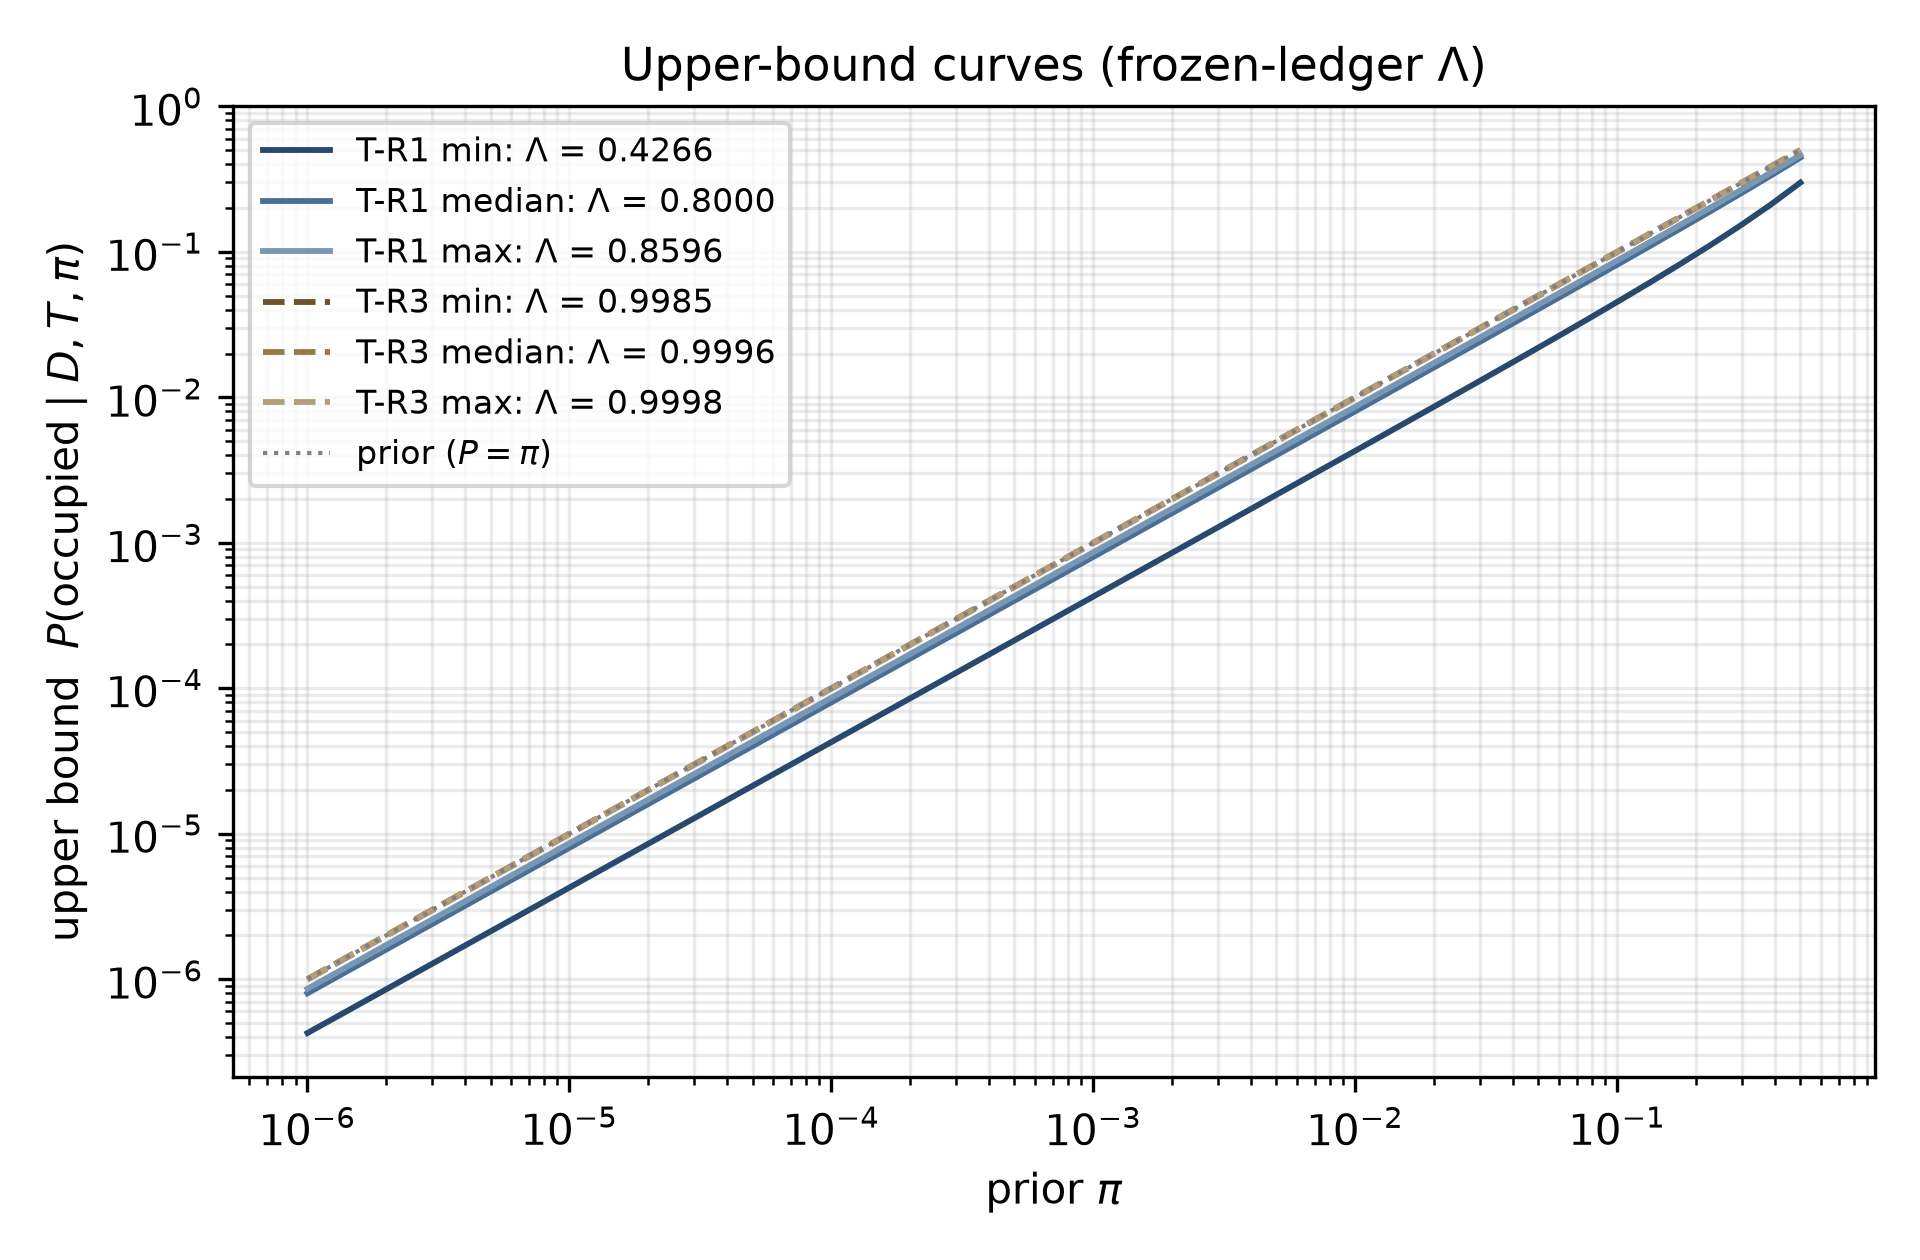
\includegraphics[width=.9\linewidth]{figs/fig1_pi_sweep.png}
\par\smallskip{\small Figure 1: upper-bound curves P(occupied | D, T, \(\pi\)) = expit(logit \(\pi\) + ln \(\Lambda\)). Curves use the frozen-ledger \(\Lambda\) (min/median/max of T-R1 and T-R3); the dotted line is the prior P = \(\pi\). Reproduce: python3 scripts/build\_paper\_figs.py}
\end{figure}
\noindent  The "vacancy" is a curve, not a single number.\par\smallskip

\subsection*{5.4 Solar self-calibration}
\noindent In the Earth-level band T-R3 the posterior \(\approx\) the prior: the lowest technology band about which this atlas can speak is calibrated by Earth itself (\S{}4.5).\par\smallskip

\subsection*{5.5 The W1 information layer (claim=false)}
\noindent For T-W1, derived from the WISE photometry embedded in GCNS, among the 192,363 main-sequence stars with W3/W4 photometry (3,615 detection candidates already in excess, 54,498 outside the model, and 82,094 without photometry are undecidable), 191,237 have \(\Lambda\) < 1 (\(\varepsilon\) > 0) at \(\gamma\) = 0.1 --- most of them \(\Lambda\) = 0, i.e. a Dyson sphere would have been detected in every T\_DS interval --- and 1,126 are insensitive with \(\Lambda\) = 1\footnote{\texttt{data/phase2/lambda\_ledger.json} (lambda\_W1\_g0.1). The \(\Lambda\) < 1 count includes stars with \(\Lambda\) = 0.}. This is physically correct: the Sun at 10 pc has a 12 \(\mu\)m photospheric flux of 1.9 Jy, whereas a \(\gamma\) = 0.1, 300 K partial Dyson sphere radiates 90 Jy. But because the G3(ii) anchor failed, this derivation carries no claim status and is provided in v1 as an information layer (off by default, with an "anchor not established" badge).\par\smallskip


\section*{6. Three-axis atlas}

\subsection*{6.1 Join rates}
\noindent Reachability was imported from the EMBARK reachability atlas v1 (37,498 stars) by DR3 source\_id: \textbf{14,799} are in GCNS (4.45\%), the remaining 22,699 lie beyond 100 pc and are outside the population (noted only), and 317,772 GCNS stars (95.55\%) are reachability-\textbf{undecidable}\footnote{\texttt{data/phase4/atlas\_v1\_summary.json}.}. Settlement resources were imported from GCNS quantities (M\_G, BP\(-\)RP, WDprob), the Mamajek colour \(\rightarrow\) type classification, the NASA Exoplanet Archive (1,037 hosts, 1,545 planets), and the HWC (45 of 70 habitable-candidate rows, 35 hosts). Nothing was recomputed on any axis.\par\smallskip


\subsection*{6.2 Cross counts (no composition)}
{\scriptsize\setlength{\tabcolsep}{2.5pt}\hyphenpenalty=50 \exhyphenpenalty=50 \begin{center}\begin{tabular}{>{\raggedright\arraybackslash}p{0.581\linewidth}>{\raggedright\arraybackslash}p{0.339\linewidth}}
Condition & Stars \\
\hline
EMBARK flyby-reachable (any cell) \(\wedge\) T-R1 bound & \textbf{815} \\
same \(\wedge\) T-R3 bound & 108 \\
EMBARK rendezvous-reachable \(\wedge\) T-R1 bound & 311 (of 2,339 rendezvous-reachable) \\
T-R1 bound (1,554) but outside EMBARK & 739 \\
T-R1 bound \(\wedge\) S1 (FGK main sequence) / S2 (all main sequence) & 633 / 1,406 \\
T-R1 bound \(\wedge\) known planet host & 136 \\
\end{tabular}\end{center}}
\noindent Accounting: 1,554 = 815 + 739. The distribution of \(\Lambda\) is the same in every EMBARK cell (the vacancy bound is set by the coverage structure of the rows and is independent of reachability). The conditional clause of every cell is attached in the atlas JSON.\par\smallskip

\subsection*{6.3 Settlement-resource slider}
\noindent S1 narrow (FGK main sequence, Mamajek classes F0--K5): 43,119 stars; S2 all main-sequence types: 283,526; S3 resource-broad (all stars): 332,571. The slider is a function selecting the displayed star set, not a criterion, and does not affect the vacancy or reachability values. Narrow habitability (liquid water, temperature) is not used as a criterion.\par\smallskip

\subsection*{6.4 HWC cross-reference table (not a composition)}
\noindent Sixteen HWC habitable-candidate hosts carry a T-R1 bound (e.g. the host of Proxima Cen b, \(\Lambda\) = 0.819, EMBARK-reachable; the host of Ross 128 b, \(\Lambda\) = 0.860, outside EMBARK). Nineteen hosts, including TRAPPIST-1, LHS 1140, and TOI-700, lie outside every radio field and are vacancy-undecidable. Being a habitable candidate and carrying a vacancy bound are independent imported quantities; the table cross-references and does not compose them.\par\smallskip

\section*{7. Discussion}

\subsection*{7.1 Interpretation and scope}
\noindent The results of this paper are meaningful only within four limits. First, this is a survey, not a proof: evidence of absence is limited and does not prove the absence of occupation. Second, a vacancy bound is not a settlement permit: no inference of the absence of occupation, nor of the legitimacy of settlement, can be drawn from this product. Third, the HWC cross-reference table is not a composition: no quantity in this paper multiplies habitable candidacy by a vacancy bound. Fourth, 1/N and the star-level posterior are different quantities, and their numerical proximity (\S{}4.3(c)) is coincidental. For the same reasons, the values presented here carry no meaning apart from their conditional clause (band, survey set, \(\pi\)); compressing them into a single number or a ranking, forming products or weighted sums across the three axes, counting undecidable stars as vacant, and using this product to justify settlement, contact, or transmission all lie outside the scope of the method. The W1 information layer has no established anchor and is not used for vacancy claims.\par\smallskip

\subsection*{7.2 Limitations and outlook}
\begin{itemize}\setlength{\itemsep}{1pt}
\item \textbf{Unpublished observations}: the BL open archive holds unpublished observations (C/X band etc.) of 1,530 GCNS stars; publication of limits could move them from undecidable (d) to decidable. UWL, optical lasers, and transients remain on the extension shelf.
\item \textbf{Independence assumptions}: independence of f\_pipe across observations is the same premise as Price et al. (2020), but correlation effects may remain outside the sensitivity range U[0.3, 0.8].
\item \textbf{Re-anchoring W1}: passive (publication of a per-star Hephaistos table, or an independent anchor at DR4 v1.1).
\item \textbf{DR4 merge (2026-12-02)}: the stellar basis will be replaced by DR4 and only the distance-dependent part of the \(\varepsilon\) ledger recomputed for v1.1 (synchronised with EMBARK v1.1).
\item \textbf{Population horizon}: GCNS is limited to 100 pc; most of the 288,315 WS20 stars (beyond 100 pc) are outside this atlas's population.
\end{itemize}

\section*{Appendix A --- \(\varepsilon\) factor table, receiver coverage, and the common \(\nu\) grid}
\noindent Transcribed from \S{}2 of the pre-registration (b) (\url{doi:10.5281/zenodo.22067884}): EIRP50, beam response, receiver coverage (L [1.10,1.20]\(\cup\)[1.34,1.90], S [1.80,2.30]\(\cup\)[2.36,2.80], P [2.60,3.45] GHz), common \(\nu\)-grid boundaries \{1.10, 1.20, 1.34, 1.80, 1.90, 2.30, 2.36, 2.60, 2.80, 3.45\}, f\_pipe 0.5, the 13-point f\_ill grid, 20 T\_DS intervals, k = 3, S/N \(\geq\) 3.5, main-sequence selection, Mamajek table sha256 1de2edee\ldots{}, WISE zero points.\par\smallskip

\section*{Appendix B --- Method record and AI disclosure}
\noindent Three roles: the human (Yukie Maeda) --- direction, gate rulings, all final decisions at branch points; chat Claude --- staff officer, independent recomputation (the second G2 path), literature cross-checks; Claude Code (Fable 5) --- execution. Operational record: 8 rulings (\#1 band set A--F; \#2 pre-registration (b) revisions; \#3 deviation, criterion revision; \#4 acceptance of failure and demotion; \#5 seven referred items; \#6 approval of the outline; \#7 conditional approval of report (2); \#8 pre-publication style and format), 2 stops (G3(i)(b), G3(ii) --- both correct, resumed by ruling), 1 deviation, 1 failed anchor, 5 self-reports (the addendum omission, the BL tally, the log path string, E-7, E-8). Error ledger r1 (E-1--E-8). This internal verification is not a substitute for human peer review.\par\smallskip

\section*{Appendix C --- Undecidable accounting (three axes)}
{\scriptsize\setlength{\tabcolsep}{2.5pt}\hyphenpenalty=50 \exhyphenpenalty=50 \begin{center}\begin{tabular}{>{\raggedright\arraybackslash}p{0.485\linewidth}>{\raggedright\arraybackslash}p{0.354\linewidth}>{\raggedright\arraybackslash}p{0.081\linewidth}}
Axis & Undecidable & Fraction \\
\hline
Vacancy (radio, three bands; outside all fields) & 330,984 & 99.52\% \\
Vacancy (W1) & extension shelf (information layer) & --- \\
Reachability (outside EMBARK) & 317,772 & 95.55\% \\
Settlement resources (no photometry) & 8,261 & 2.48\% \\
\end{tabular}\end{center}}

\section*{Appendix D --- Reproducibility and data release}
\noindent Regeneration: \texttt{python3 src/vacancy/build\_ledger.py} (3 s) / Figure 1: \texttt{python3 scripts/build\_paper\_figs.py} \(\rightarrow\) \texttt{scripts/export\_g2.py} \(\rightarrow\) \texttt{python3 src/vacancy/aggregate.py} (\(\approx\)10 min) \(\rightarrow\) \texttt{scripts/g3\_i\_ws20\_price.py} / \texttt{g3\_ii\_hephaistos.py} / \texttt{g3\_iii\_solar\_selftest.py} \(\rightarrow\) \texttt{python3 src/vacancy/build\_atlas.py}. Unit tests: \texttt{python3 -m unittest tests.test\_epsilon} (14 tests). Released files: the \(\varepsilon\) ledger (\texttt{ledger\_v0.json}, formula version eps-v0.2), the \(\Lambda\) ledger (\texttt{lambda\_ledger.json}), the three-axis atlas (\texttt{atlas\_v1.json}), radio-row provenance (\texttt{radio\_obs\_v0.json}), the G1/G2/G3 reports, frozen copies of the NEA and HWC inputs, all scripts, error ledger r1, and the SHA-256 manifest (\texttt{MANIFEST.json}). Pre-registration (a) commit 10a01e710854b69344651ed6ba016ab303c9d124; (b) \url{doi:10.5281/zenodo.22067884.}\par\smallskip

\section*{Acknowledgements}
\noindent This work has made use of data from the European Space Agency (ESA) mission Gaia (\url{https://www.cosmos.esa.int/gaia}), processed by the Gaia Data Processing and Analysis Consortium (DPAC, \url{https://www.cosmos.esa.int/web/gaia/dpac/consortium}). Funding for the DPAC has been provided by national institutions, in particular the institutions participating in the Gaia Multilateral Agreement. This research has made use of the NASA Exoplanet Archive, which is operated by the California Institute of Technology, under contract with the National Aeronautics and Space Administration under the Exoplanet Exploration Program. This research has made use of the VizieR catalogue access tool, CDS, Strasbourg, France (DOI: 10.26093/cds/vizier). The Habitable Worlds Catalog is maintained by the Planetary Habitability Laboratory @ UPR Arecibo. Observation metadata from the Breakthrough Listen open data archive (seti.berkeley.edu/opendata) were used.\par\smallskip

\section*{References}
\noindent [1] Price D. C. et al. 2020, AJ 159, 86. [2] Wlodarczyk-Sroka B. S., Garrett M. A., Siemion A. P. V. 2020, MNRAS 498, 5720. [3] Enriquez J. E. et al. 2017, ApJ 849, 104. [4] Isaacson H. et al. 2017, PASP 129, 054501. [5] Lebofsky M. et al. 2019, PASP 131, 124505. [6] Suazo M. et al. 2022, MNRAS 512, 2988. [7] Suazo M. et al. 2024, MNRAS 531, 695. [8] Wright J. T. et al. 2014, ApJ 792, 26; 792, 27. [9] Griffith R. L. et al. 2015, ApJS 217, 25. [10] Wright J. T., Kanodia S., Lubar E. 2018, AJ 156, 260. [11] Grimaldi C. 2017, Sci. Rep. 7, 46273. [12] Gaia Collaboration, Smart R. L. et al. 2021, A\&A 649, A6. [13] Gaia Collaboration 2016, A\&A 595, A1; 2021, A\&A 649, A1; 2023, A\&A 674, A1. [14] Brandt T. D. 2021, ApJS 254, 42. [15] Bailer-Jones C. A. L. et al. 2018, AJ 156, 58. [16] Pecaut M. J., Mamajek E. E. 2013, ApJS 208, 9. [17] Wright E. L. et al. 2010, AJ 140, 1868; Cutri R. M. et al. 2014, VizieR II/328; Marocco F. et al. 2021, ApJS 253, 8. [18] Jarrett T. H. et al. 2011, ApJ 735, 112. [19] Sullivan W. T., Brown S., Wetherill C. 1978, Science 199, 377; Saide R. C. et al. 2023, MNRAS 522, 2393. [20] Sheikh S. Z. et al. 2019, ApJ 884, 14. [21] NASA Exoplanet Archive, Planetary Systems Composite Parameters, \url{doi:10.26133/NEA12} (retrieved 2026-08-23). [22] Habitable Worlds Catalog, PHL @ UPR Arecibo (retrieved 2026-08-23). [23] Maeda Y. 2026a, Zenodo, \url{doi:10.5281/zenodo.22067884} (pre-registration (b)); Maeda Y. 2026b, WAKE, Zenodo, \url{doi:10.5281/zenodo.21966305}; Maeda Y. 2026c, EMBARK, Zenodo, \url{doi:10.5281/zenodo.22059576.}\par\smallskip
\end{document}
